%!TEX root = volumeFinal.tex 
\chapter{\label{chap:ativ}Análise e Projeto}

\section{Jogos}
 Jogos eletrônicos são muito populares, principalmente pela grande quantidade de gêneros, existem jogos de ação, aventura, esportes, estratégia, entre outros. Hoje em dia, os jogos buscam que quem jogue consiga ficar imerso no dentro do jogo, sem conseguir identificar um padrão nos jogadores fictícios, pois se não o jogo deixa de ser tão interessante. Para que isso aconteça, a IA é associada a diversos jogos, e é comum pensar que quanto mais complexa a IA aplicada dentro do jogo mais difícil jogo irá ficar, mas isso nem sempre é verdade, nem sempre IA complicadas terão melhor desempenho do que as mais simples, uma boa IA dentro do jogo é feita a partir de determinar o comportamento certo para os algoritmo certos \cite{millington2009artificial}.
 
 \subsection{Jogos de estratégia em tempo real}
 
 Jogos de estratégia em tempo real, também conhecido por \textit{real-time strategy games} (RTS), é um subgênero de jogos de estratégia, onde os jogadores precisam construir uma base com uma economia, ganhando recursos, construindo edificações, treinando unidades de ataques e tecnologias para elas, tudo isso com o objetivo de destruir uma ou mais bases inimigas \cite{ontanon2013survey, buro2012real}. 
 
 Existem algumas diferenças entre jogos RTS e jogos de tabuleiro, como xadrez. Estas diferenças são \cite{ontanon2013survey}:
 
 \begin{itemize}
 	\item movimentos simultâneos, jogadores realizam jogadas ao mesmo tempo;
 	\item tempo real, cada jogador deve realizar suas ações em um curto espaço de tempo;
 	\item parcialmente observável, na maioria dos jogos RTS, o jogador só consegue enxergar parte do ambiente;
 	\item não-determinístico, nem sempre uma ação realizada resulta na saída esperada; e
 	\item complexidade, o espaço de estados e o número de ações possíveis é muito grande.
 \end{itemize} 
 
 
 Pelo fato de existirem essas diferenças, não é possível traduzir automaticamente as técnicas padrões dos jogos de tabuleiro para jogos RTS sem algum tipo de abstração ou simplificação \cite{ontanon2013survey}.
 
\subsection{MicroRTS}  
 
 Um exemplo deste gênero é o MicroRTS\footnote{https://github.com/santiontanon/microrts}, uma simplificação do jogo Starcraft\footnote{http://us.battle.net/sc2/pt/}, feita por Santiago Ontañón \cite{ontanon2013combinatorial} em Java. O MicroRTS foi desenvolvido para fins acadêmicos, com o intuito de aplicar e desenvolver técnicas de IA e para servir como prova de conceito para as técnicas criadas.
 
 \begin{figure}[ht]
 	\centering
 	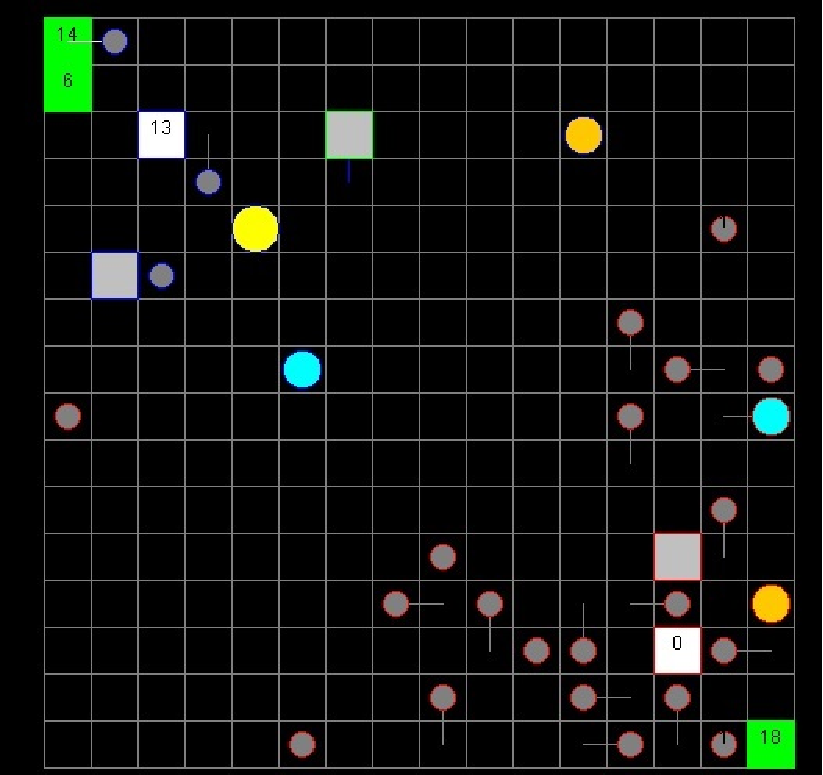
\includegraphics[width=0.5\textwidth]{fig/microrts.pdf}
 	\caption{Um exemplo de tela do MicroRTS}
 	\label{fig:microrts}
 \end{figure} 
 
O MicroRTS consiste em dois jogadores tentando destruir a base adversaria. Para destruir com o inimigo é preciso eliminar cada unidade e edificações adversarias. A Figura~\ref{fig:microrts} mostra uma tela do jogo. Existem quatro tipos de unidades no jogo, são elas:
  
\begin{itemize}
 	\item \textit{worker}, é responsável por coletar recursos e construir as edificações. Esta unidade também consegue lutar, mas possui um dano muito baixo;
 	\item \textit{heavy}, unidade que pode apenas atacar. Ela possui um alto poder de ataque, mas sua velocidade é lenta;
 	\item \textit{light}, unidade que pode apenas atacar. Ela possui um baixo poder de ataque, mas sua velocidade é rápida; e
 	\item \textit{ranged}, unidade que pode apenas atacar. Ela possui um ataque de longa distância. 
\end{itemize} 
 
Para adquirir as unidades é preciso das edificações e recursos. Existem três tipos de edificações, são elas:

\begin{itemize}
	\item base, a base é a edificação principal, ela é responsável pela criação dos \textit{workers}, e nela também é guardado os recursos coletados pelos \textit{workers};
	\item quartel, o quartel é responsável pela criação das unidades de ataque \textit{heavy}, \textit{light} e \textit{ranged}. Ela pode ser construída pelos \textit{workers} usando recursos; e
	\item base de recurso, na base de recurso são coletados os recursos pelos \textit{workers}, os a base de recursos é finitos para ser coletada.
\end{itemize}  

No início do jogo, cada jogador inicia com uma base, um \textit{worker} e uma base de recurso para coletar. Todas as unidades podem ser atacas menos a base de recursos. 
 
No ambiente há algumas estratégias implementadas, cada estratégia possui variações dos algoritmos. Algumas das estratégias são:
 \begin{itemize}
 	\item \textit{Minimax Alpha-Beta Search Strategies} - O que muda entre as técnicas é o jeito com que é feito a expansão do grafo.
 	\item \textit{Monte Carlo Search Strategies} - Executa jogadas aleatórias para planejar e após utiliza uma heurística para determinar em qual caminho seguir.
 \end{itemize}
 
 A plataforma já foi utilizada para aplicar técnica de IA. Por esse motivo a utilização dela se torna viável para a realização deste trabalho. 
Nela é possível observar que o fator de ramificação pode ser muito alto dependendo do cenário do jogo.

\subsection{Arquitetura do MicroRTS}

A arquitetura do MicroRTS é composta por 4 componentes principais: O Jogo em si, onde são feitas todas as ações dos jogos. As unidades, onde todas as ações de cada unidade podem ser controladas e acessadas, por exemplo, saber onde está cada unidade inimiga. A Interface gráfica, responsável pela representação gráfica do jogo. E a Inteligência Artificial, onde pode ser acoplado a IA que desejar, a plataforma já possui algumas como foi dito anteriormente. A imagem \ref{fig:pacotes} representa os componentes.

 \begin{figure}[ht]
 	\centering
 	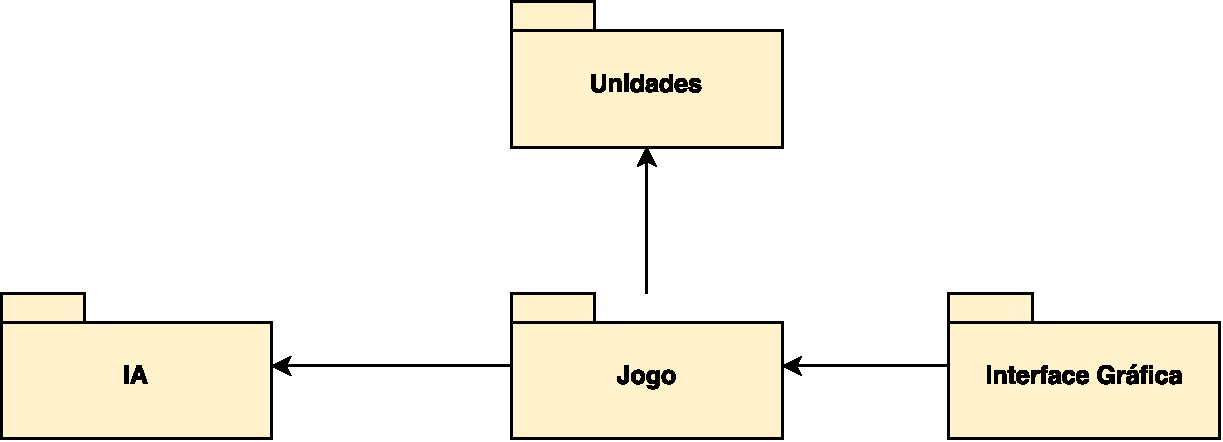
\includegraphics[width=0.4\textwidth]{fig/pacotes.pdf}
 	\caption{Arquitetura MicroRTS}
 	\label{fig:pacotes}
 \end{figure} 
 
\section{Descrição do Projeto}
 
Para realizar a implementação de uma IA para acoplar no MicroRTS, é preciso conhecer as classes responsáveis por cada componente. A Figura \ref{fig:classes} ilustra as principais classes presentes no jogo. A Classe \textit{GameVisualSimulation} é a interface entre os componentes do jogo e o usuário. A classe \textit{GameState} e \textit{PhysicalGameState}, são responsáveis pelo controle das ações das unidades, e pelo controle do mapa e das unidades dentro dele, respectivamente. A classe \textit{UnitTypeTable} é onde cada unidade é associada as ações possíveis no jogo. A Classe \textit{PhysicalGameStatePanel} é responsável pela interface gráfica. E por fim a classe \textit{AHTN} é onde minha proposta de solução será acoplada ao jogo.
 
  \begin{figure}[ht]
  	\centering
  	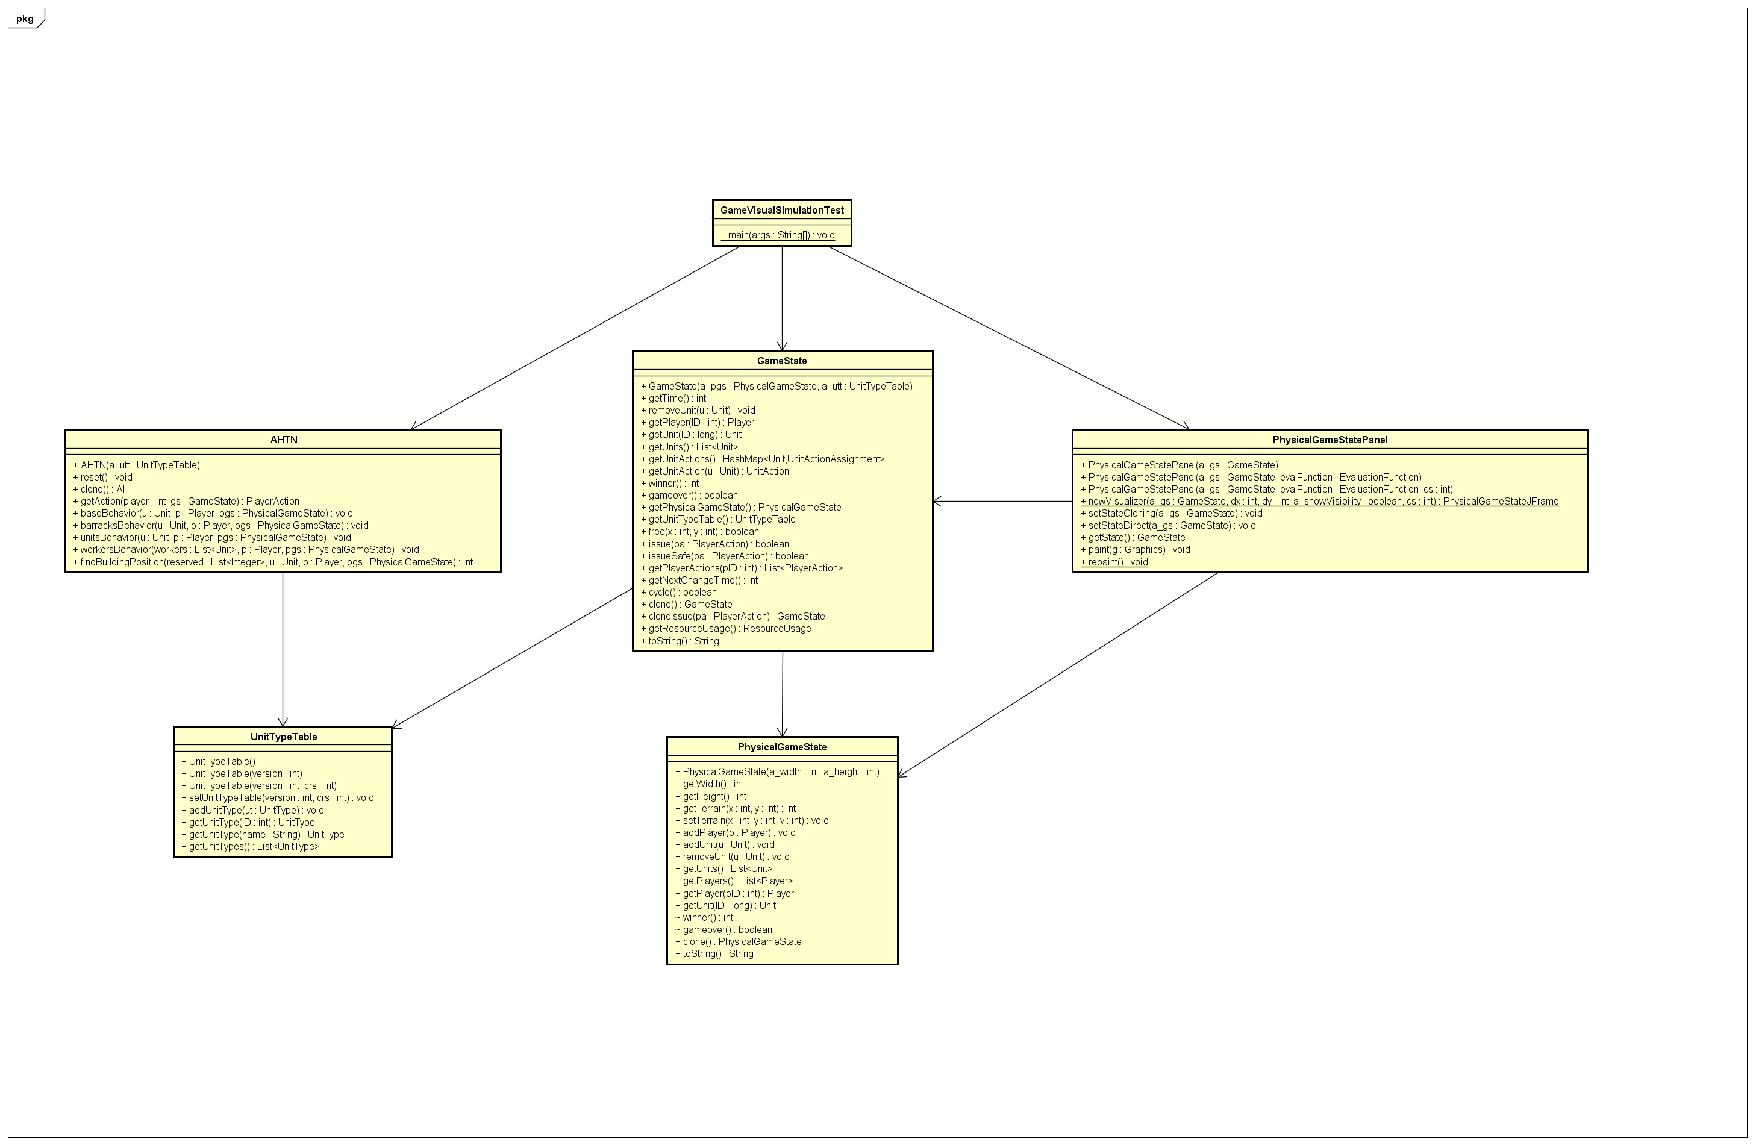
\includegraphics[width=1\textwidth]{fig/classes.pdf}
  	\caption{Classes do MicroRTS}
  	\label{fig:classes}
  \end{figure} 

A Figura~\ref{fig:sequencia} apresenta o diagrama de sequência, para entender o funcionamento das classes citadas acima. Os passos de 1 a 6 são apenas para criação dos objetos que serão utilizados pelo jogo. No passo 7 é gerado a ação que deve ser executado no momento atual do jogo, já no passo 8 é confirmado se foi encontrado alguma ação que possa ser executada. No passo 9 a tela é desenha novamente com a atualização das jogadas. Existe um laço do passo 7 até o 9, pois são onde são geradas as ações, esse laço acaba quando termina o tempo limite de jogo, ou algum jogador vence. O diagrama mostra a geração da jogada para apenas um jogador, mas a forma como as jogadas são geradas é da mesma forma como a apresentada. O algoritmo de AHTN irá ser implementado dentro do método $getAction$, e portanto estará presente no passo 7 do diagrama.

\begin{figure}[ht]
  	\centering
  	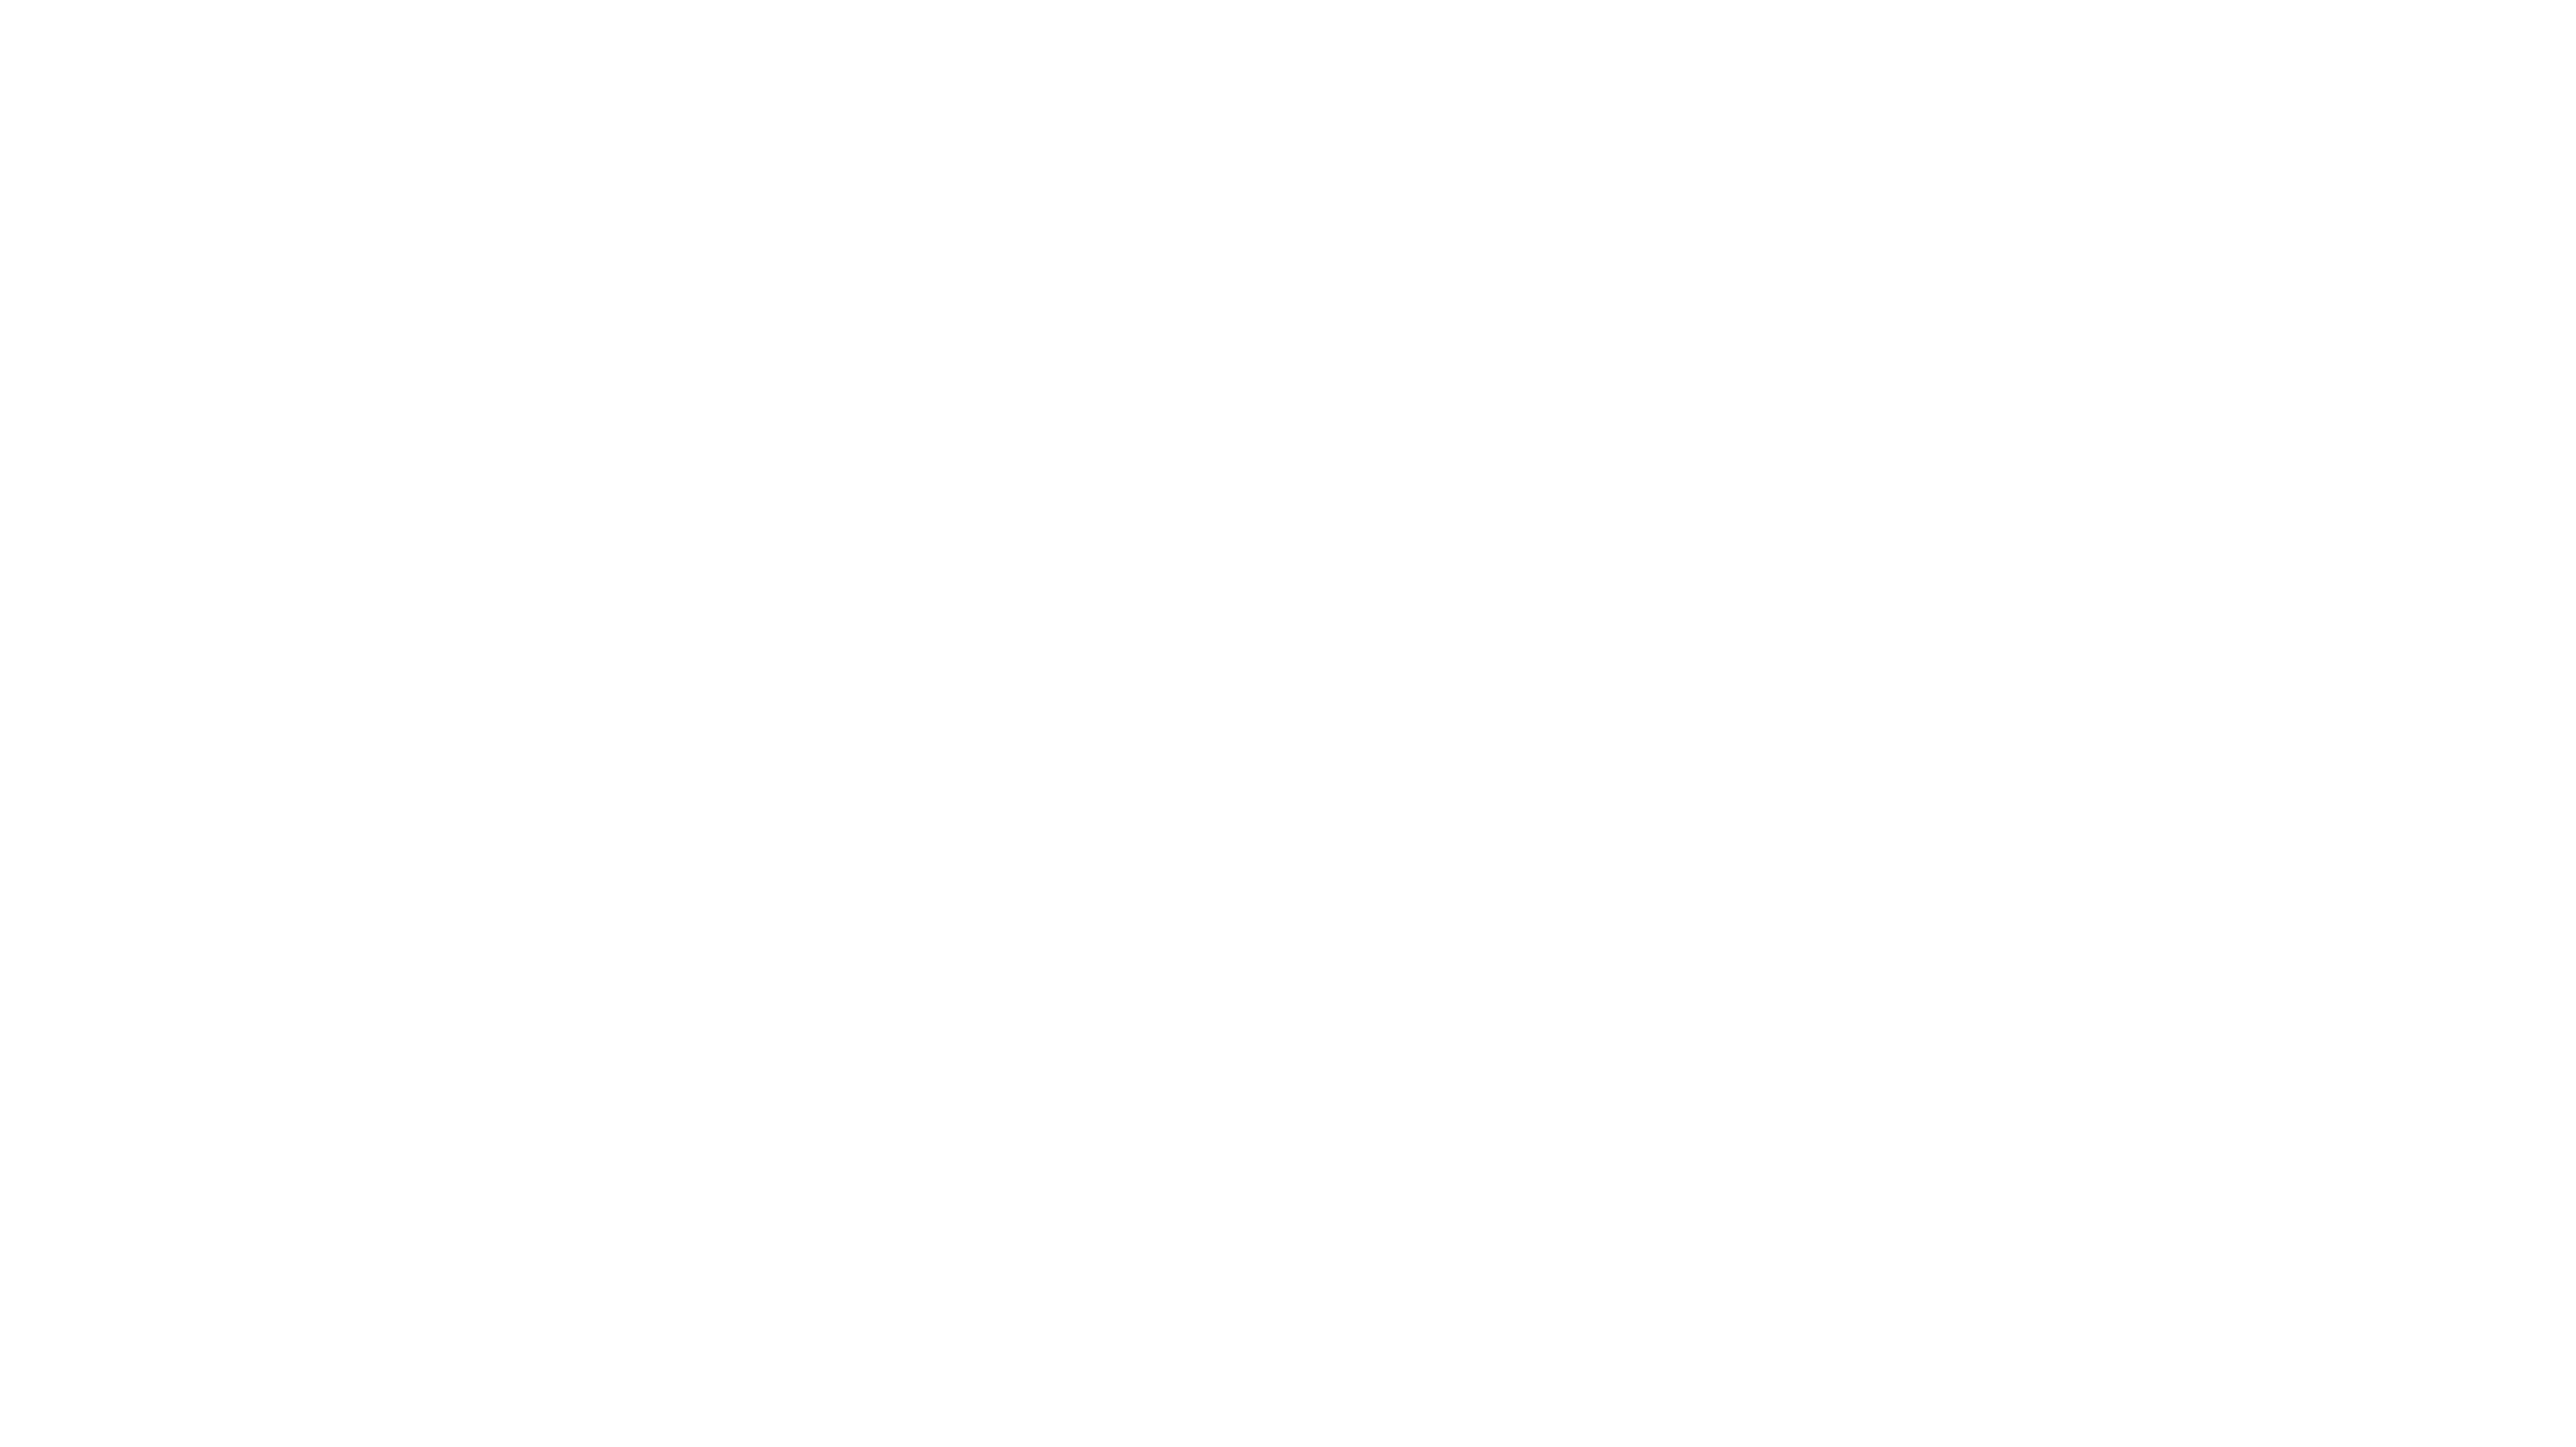
\includegraphics[width=1\textwidth]{fig/diagramaSequencia.pdf}
  	\caption{Diagrama de sequência}
  	\label{fig:sequencia}
\end{figure}


\section{Cronograma}

Para a próxima etapa do projeto do Trabalho de Conclusão, foi proposto o plano das atividades apresentado no diagrama de Gantt com a respectiva legenda.

\begin{itemize}
\item Tarefa 1 - Escrita do TC II.
\item Tarefa 2 - Desenvolvimento do dominio.
\item Tarefa 3.1 - Implementação do algoritmo AHTN.
\item Tarefa 3.2 - Testar e corrigir possíveis erros da implementação.
\item Tarefa 4 - Criação dos \textit{benchmark}.
\item Tarefa 5 - Integrar o algoritmo de \textit{q-learning} a implementação. 
\item Tarefa 6 - Realizar a comparação com as outras abordagens. 
\item Tarefa 7 - Preparar a apresentação. 
\end{itemize}

\begin{ganttchart}{1}{21}
	\gantttitle{Volume Final TCI}{21} \\
	\gantttitlelist{6,...,12}{3} \\
	\ganttgroup{TC II}{6}{20} \\	
	\ganttmilestone{Entrega do volume Final TCI}{3} \ganttnewline	
	\ganttbar{Tarefa 1}{7}{20} \\	
	\ganttbar{Tarefa 2}{7}{8} \\
	\ganttbar{Tarefa 3.1}{9}{10} \\	
	\ganttbar{Tarefa 3.2}{11}{12} \\	
	\ganttbar{Tarefa 4}{13}{14} \\
	\ganttbar{Tarefa 5}{15}{16} \\
	\ganttbar{Tarefa 6}{17}{18} \\	
	\ganttbar{Tarefa 7}{19}{20} \\	
	\ganttmilestone{Entrega Volume Final}{20} \ganttnewline
	%\ganttlinkedgroup{Task 3}{2}{3}
	%\ganttlinkedbar{Task 3}{3}{7} \ganttnewline
%	%\ganttmilestone{Milestone}{7} \ganttnewline
%	%\ganttbar{Final Task}{8}{12}	
%	\ganttlink{elem2}{elem8}
%	\ganttlink{elem5}{elem6}	
%	\ganttlink{elem3}{elem6}
%	\ganttlink{elem4}{elem7}
%	\ganttlink{elem6}{elem7}
%	\ganttlink{elem8}{elem9}
\end{ganttchart}

